\section{Results}
\label{Benchmarking:Results}

We provide now the results of the execution of the privacy filters, with the configuration specified in the previous section. For each filter, we present summary tables with the disclosure risk and information loss estimates for each parameterization, as well as plots showing the evolution of both measurements against the number of instances processed.

\subsection{Noise addition}
\label{Benchmarking:Results:Noise}

\begin{minipage}[t]{0.5\textwidth}
	\begin{flushleft}
	\begin{table}[H]
		\centering
		\begin{tabular}{@{}rrrr@{}}
			\toprule
			$a$ & $c$ & \multicolumn{1}{c}{DR} & \multicolumn{1}{c}{IL} \\ \midrule
			0.1 & 0.0 & 0.956	& 1123.97 \\
			0.25 & 0.0 & 0.889 & 7024.83 \\
			0.5 & 0.0 & 0.774	& 28099.33 \\
			0.75 & 0.0 & 0.596 & 63223.50 \\
			1.0 & 0.0 & 0.430 & 112397.34 \\ \bottomrule
		\end{tabular}
		\caption[Noise addition DR \& IL estimations (\texttt{RandomRBFGenerator}).]{Noise addition IL \& DR estimations for all considered parameterizations with the \texttt{RandomRBFGenerator}.}
		\label{table:results-rbf-noise-addition}
	\end{table}
	\end{flushleft}
\end{minipage}
\begin{minipage}[t]{0.5\textwidth}
	\begin{flushright}
	\begin{table}[H]
		\centering
		\begin{tabular}{@{}rrrr@{}}
			\toprule
			$a$ & $c$ & \multicolumn{1}{c}{DR} & \multicolumn{1}{c}{IL} \\ \midrule
			0.1  & 0.0 & 1.000 & 50741.41   \\
			0.25 & 0.0 & 1.000 & 317133.83  \\
			0.5  & 0.0 & 0.996 & 1268535.34 \\
			0.75 & 0.0 & 0.919 & 2854204.53 \\
			1.0  & 0.0 & 0.742 & 5074141.39 \\ \bottomrule
		\end{tabular}
		\caption[Noise addition DR \& IL estimations (\texttt{WaveformGenerator}).]{Noise addition IL \& DR estimations for all considered parameterizations with the \texttt{WaveformGenerator}.}
		\label{table:results-wave-noise-addition}
	\end{table}
	\end{flushright}
\end{minipage}

\begin{figure}[h]
	\centering
	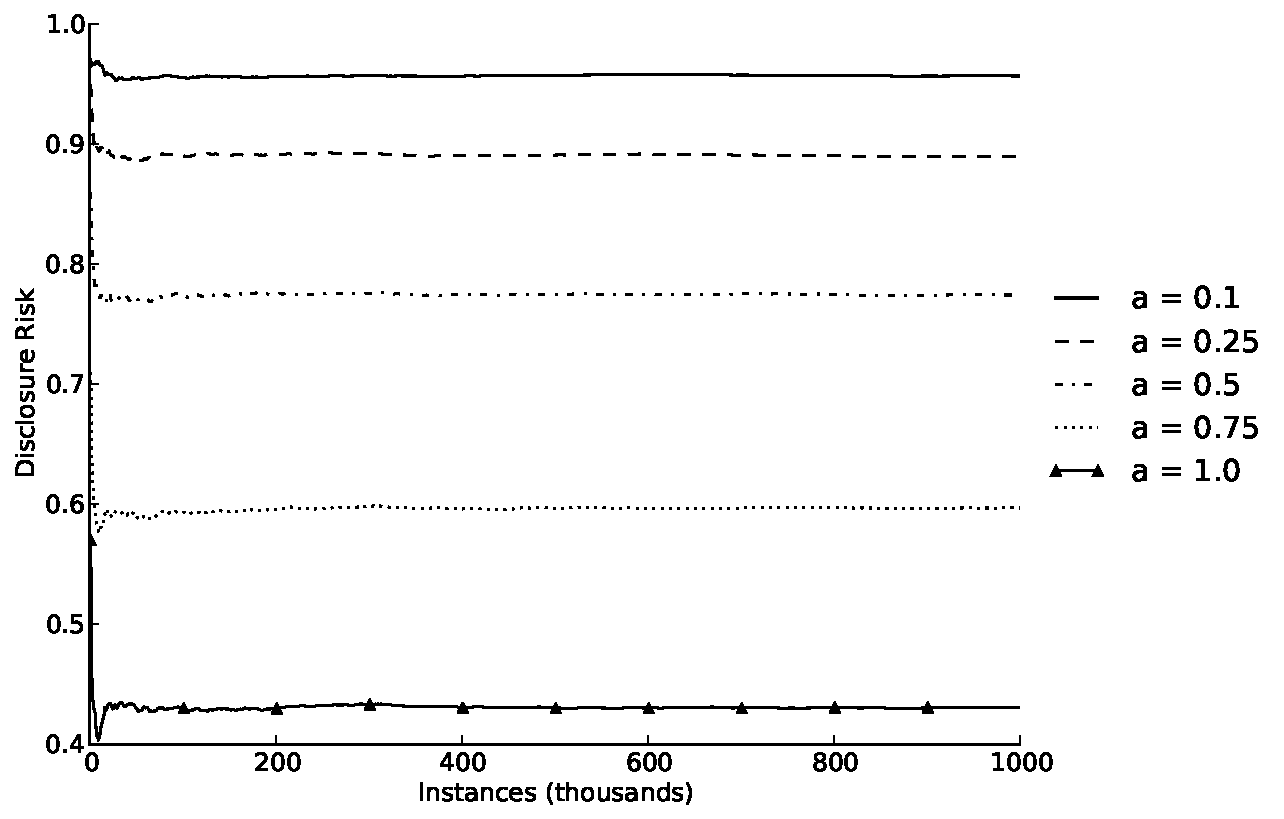
\includegraphics[width=0.9\linewidth]{figures/dr_na-random.pdf}
	\caption[Noise addition DR evaluation ($c = 0$).]{\texttt{NoiseAdditionFilter} DR evaluation using the \texttt{RandomRBFGenerator} with fixed parameter $c = 0$.}
	\label{fig:results-dr-na}
\end{figure}

\begin{figure}[h]
	\centering
	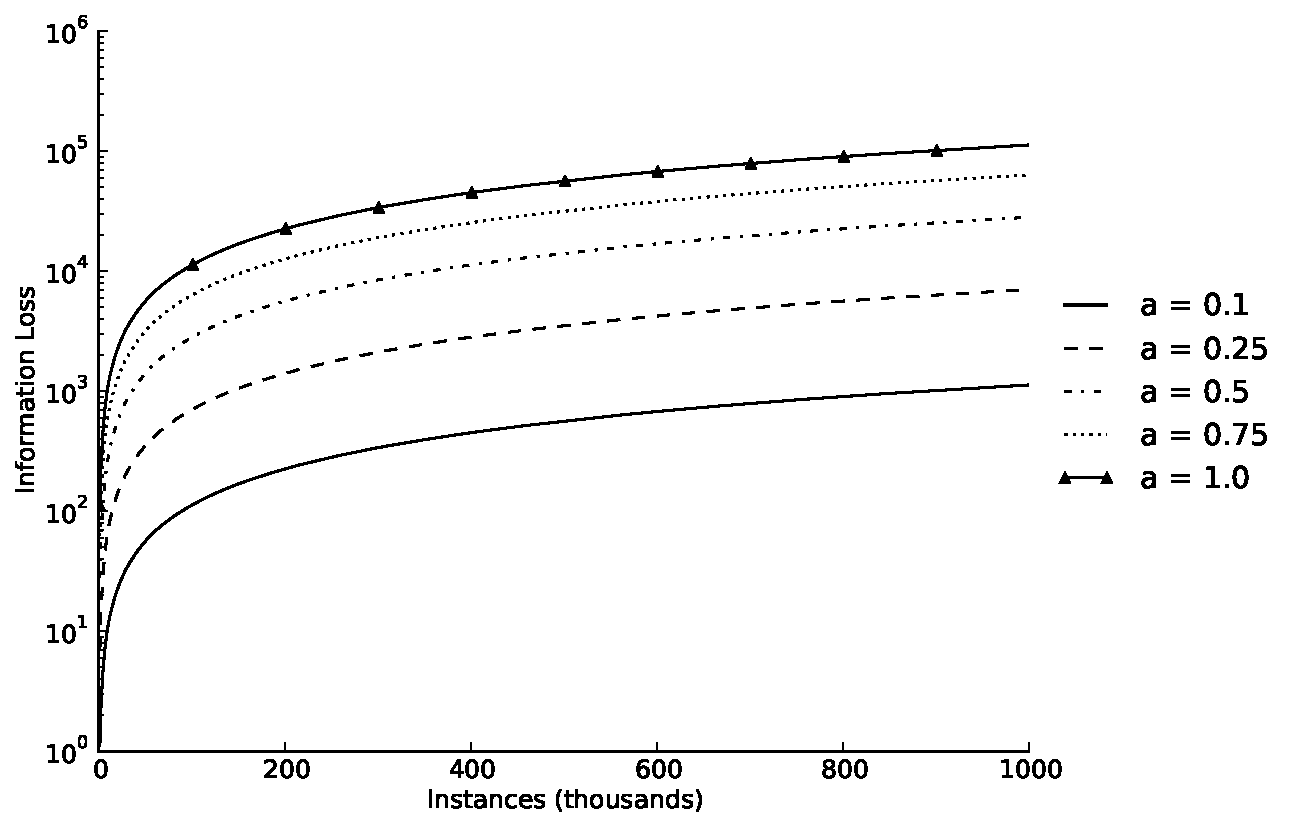
\includegraphics[width=0.9\linewidth]{figures/il-log_na-random.pdf}
	\caption[Noise addition IL evaluation ($c = 0$), logarithmic scale.]{\texttt{NoiseAdditionFilter} IL evaluation using the \texttt{RandomRBFGenerator} with fixed parameter $c = 0$, on a logarithmic scale.}
	\label{fig:results-il-log-na}
\end{figure}

\subsection{Microaggregation}
\label{Benchmarking:Results:MicroAgg}

\begin{minipage}[t]{0.5\textwidth}
	\begin{flushleft}
	\begin{table}[H]
		\centering
		\begin{tabular}{@{}rrrr@{}}
			\toprule
			$b$ & $k$ & \multicolumn{1}{c}{DR} & \multicolumn{1}{c}{IL} \\ \midrule
			100  & 3   & 0.232 & 74917.30  \\
			100  & 5   & 0.144 & 89953.68  \\
			100  & 10  & 0.089 & 101193.72 \\
			100  & 15  & 0.069 & 104952.79 \\
			100  & 20  & 0.061 & 106800.51 \\
			100  & 25  & 0.055 & 107937.42 \\
			100  & 50  & 0.041 & 110179.72 \\
			100  & 100 & 0.030 & 111313.78 \\ \bottomrule
		\end{tabular}
		\caption[Microaggregation DR \& IL estimations (\texttt{RandomRBFGenerator}).]{Microaggregation IL \& DR estimations for increasing $k$ (cluster size) and fixed buffer size $b=100$ with the \texttt{RandomRBFGenerator}.}
		\label{table:results-rbf-microaggregation}
	\end{table}
	\end{flushleft}
\end{minipage}
\begin{minipage}[t]{0.5\textwidth}
	\begin{flushright}
	\begin{table}[H]
		\centering
		\begin{tabular}{@{}rrrr@{}}
			\toprule
			$b$ & $k$ & \multicolumn{1}{c}{DR} & \multicolumn{1}{c}{IL} \\ \midrule
			100  & 3   & 0.241 & 3375656.78 \\
			100  & 5   & 0.135 & 4057649.13 \\
			100  & 10  & 0.076 & 4566550.54 \\
			100  & 15  & 0.061 & 4739204.47 \\
			100  & 20  & 0.054 & 4822716.29 \\
			100  & 25  & 0.049 & 4872587.52 \\
			100  & 50  & 0.038 & 4976718.32 \\
			100  & 100 & 0.029 & 5027574.64 \\ \bottomrule
		\end{tabular}
		\caption[Microaggregation DR \& IL estimations (\texttt{WaveformGenerator}).]{Microaggregation IL \& DR estimations for increasing $k$ (cluster size) and fixed buffer size $b=100$ with the \texttt{WaveformGenerator}.}
		\label{table:results-wave-microaggregation}
	\end{table}
	\end{flushright}
\end{minipage}

\begin{figure}[h]
	\centering
	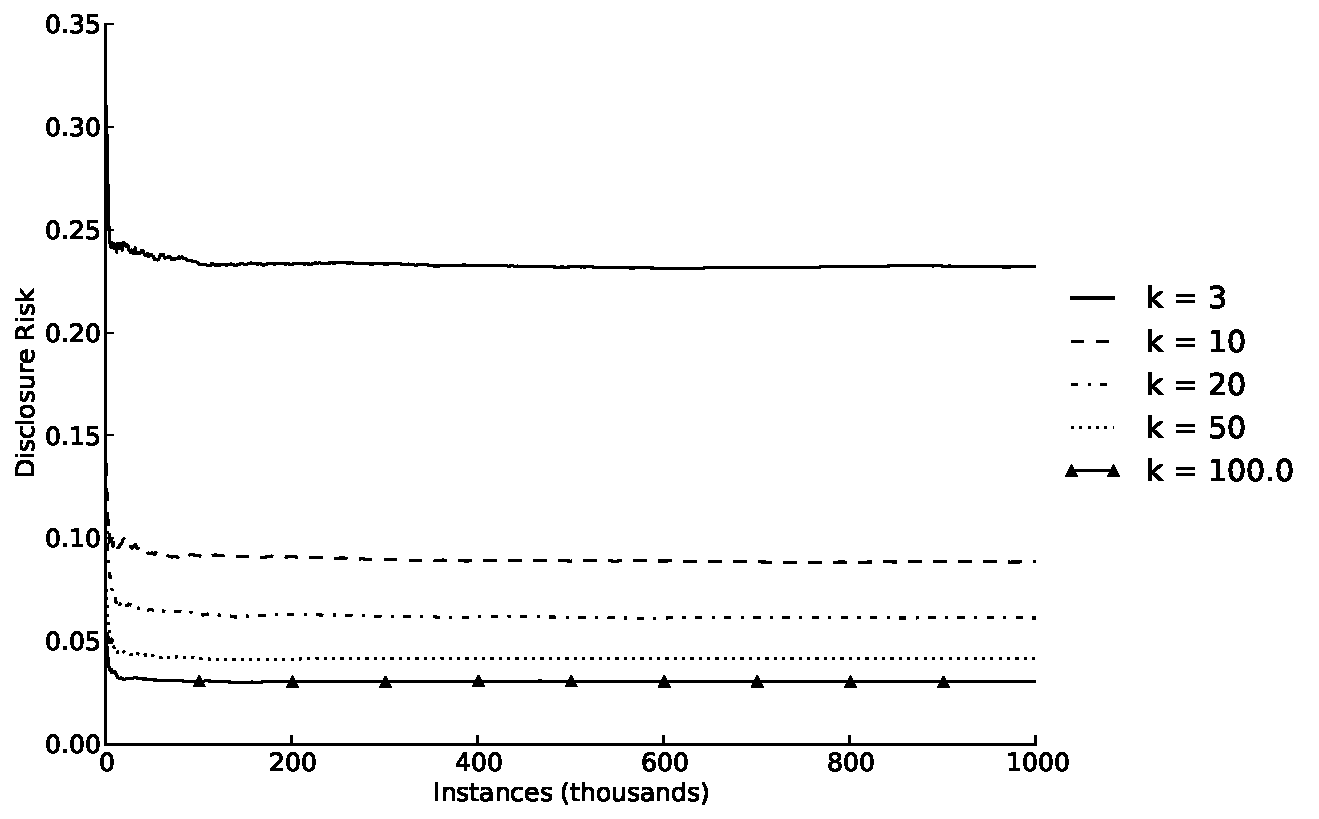
\includegraphics[width=0.9\linewidth]{figures/dr_ma-random.pdf}
	\caption[Microaggregation DR evaluation ($b = 100$).]{\texttt{MicroaggregationFilter} DR evaluation using the \texttt{RandomRBFGenerator} with fixed buffer size $b = 100$, for increasing $k$.}
	\label{fig:results-dr-ma}
\end{figure}

\begin{figure}[h]
	\centering
	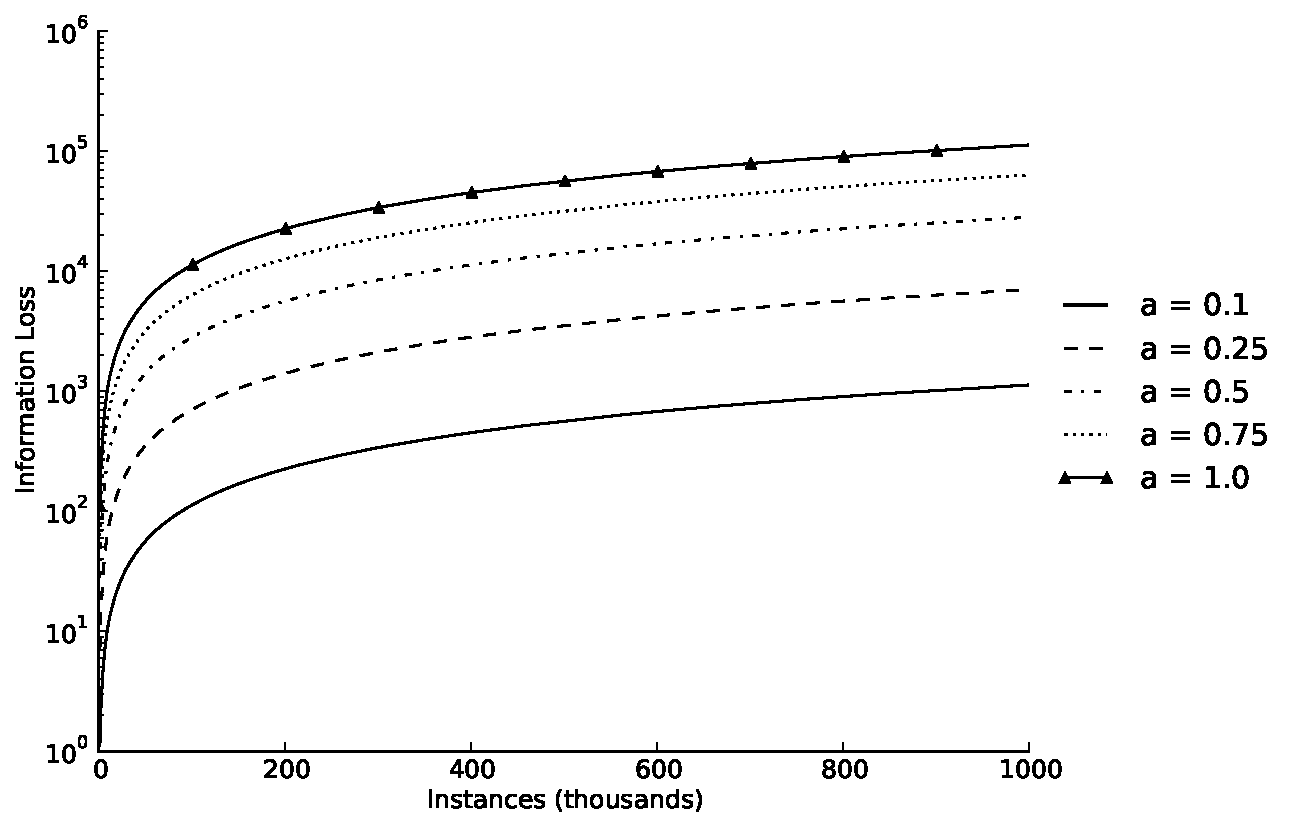
\includegraphics[width=0.9\linewidth]{figures/il-log_na-random.pdf}
	\caption[Microaggregation IL evaluation ($b = 100$), logarithmic scale.]{\texttt{MicroaggregationFilter} IL evaluation using the \texttt{RandomRBFGenerator} with fixed buffer size $b = 100$, for increasing $k$, on a logarithmic scale.}
	\label{fig:results-il-log-ma}
\end{figure}

\subsection{Rank swapping}
\label{Benchmarking:Results:RankSwap}

\begin{minipage}[t]{0.5\textwidth}
	\begin{flushleft}
	\begin{table}[H]
		\centering
		\begin{tabular}{@{}rrrr@{}}
			\toprule
			$b$ & $p$ & \multicolumn{1}{c}{DR} & \multicolumn{1}{c}{IL} \\ \midrule
			100  & 10 & 0.838 & 19136.62  \\
			100  & 25 & 0.469 & 57753.05  \\
			100  & 50 & 0.070 & 136791.17 \\
			100  & 75 & 0.036 & 178200.11 \\
			100  & 80 & 0.037 & 178685.81 \\ \bottomrule
		\end{tabular}
		\caption[Rank swapping DR \& IL estimations (\texttt{RandomRBFGenerator}).]{Rank swapping IL \& DR estimations for increasing $p$ (maximum swap range) and fixed buffer size $b=100$ with the \texttt{RandomRBFGenerator}.}
		\label{table:results-rbf-rankswap}
	\end{table}
	\end{flushleft}
\end{minipage}
\begin{minipage}[t]{0.5\textwidth}
	\begin{flushright}
	\begin{table}[H]
		\centering
		\begin{tabular}{@{}rrrr@{}}
			\toprule
			$b$ & $p$ & \multicolumn{1}{c}{DR} & \multicolumn{1}{c}{IL} \\ \midrule
			100  & 10 & 0.997 & 705196.07  \\
			100  & 25 & 0.776 & 2464673.56 \\
			100  & 50 & 0.112 & 6195304.18 \\
			100  & 75 & 0.046 & 8088473.27 \\
			100  & 80 & 0.045 & 8097619.70 \\ \bottomrule
		\end{tabular}
		\caption[Rank swapping DR \& IL estimations (\texttt{WaveformGenerator}).]{Rank swapping IL \& DR estimations for increasing $p$ (maximum swap range) and fixed buffer size $b=100$ with the \texttt{WaveformGenerator}.}
		\label{table:results-wave-rankswap}
	\end{table}
	\end{flushright}
\end{minipage}

\begin{figure}[h]
	\centering
	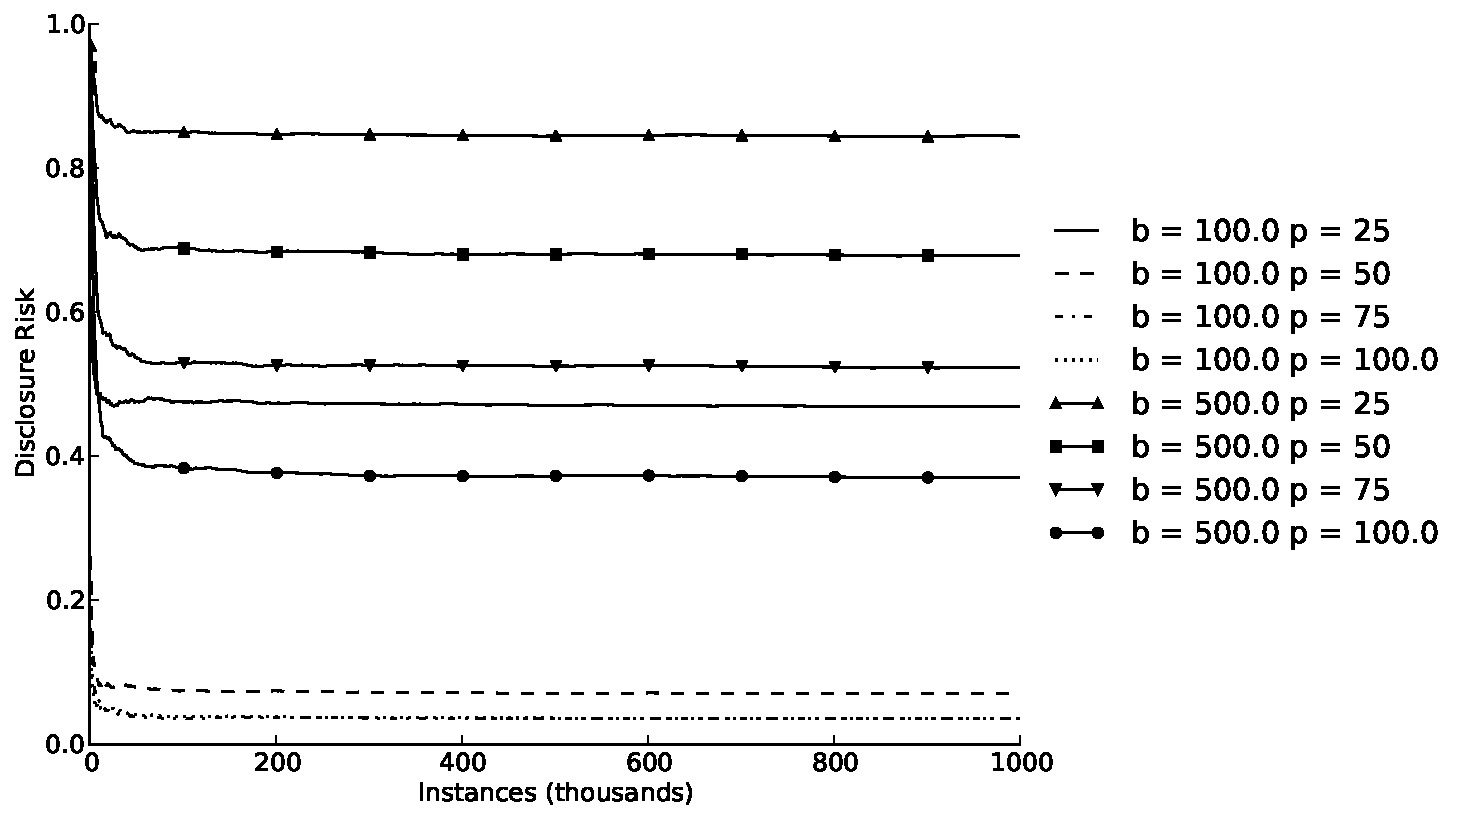
\includegraphics[width=1.0\linewidth]{figures/dr_rs-random.pdf}
	\caption[Rank swapping DR evaluation ($b = \{100,500\}$).]{\texttt{RankSwappingFilter} DR evaluation using the \texttt{RandomRBFGenerator} with buffer sizes $b = 100$ and $b = 500$, for increasing $p$.}
	\label{fig:results-dr-rs}
\end{figure}

\begin{figure}[h]
	\centering
	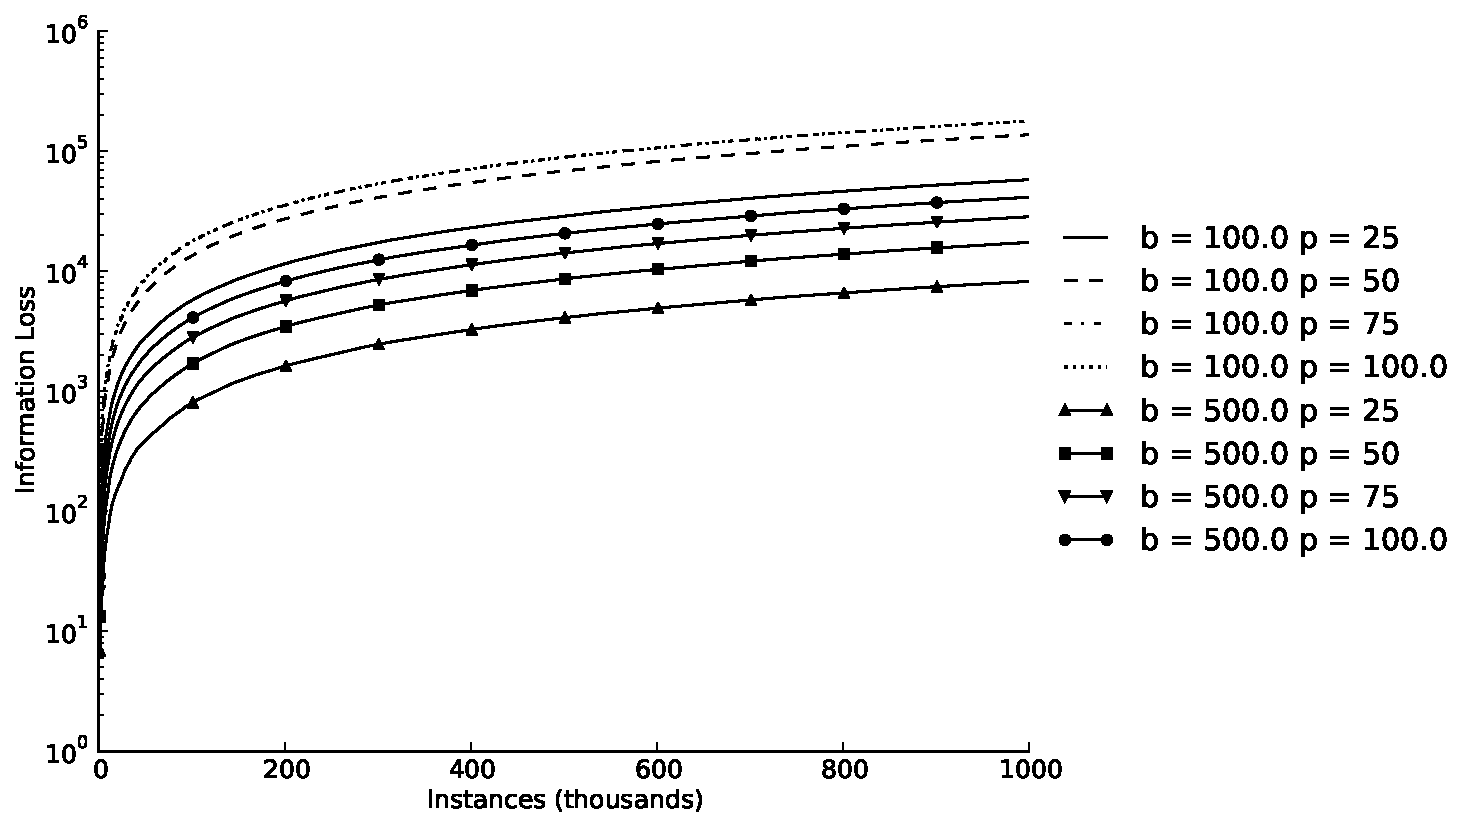
\includegraphics[width=1.0\linewidth]{figures/il-log_rs-random.pdf}
	\caption[Rank swapping IL evaluation ($b = \{100,500\}$), logarithmic scale.]{\texttt{RankSwappingFilter} IL evaluation using the \texttt{RandomRBFGenerator} with buffer sizes $b = 100$ and $b = 500$, for increasing $p$, on a logarithmic scale.}
	\label{fig:results-il-log-rs}
\end{figure}

\subsection{$\varepsilon$-Differential private microaggregation}
\label{Benchmarking:Results:DiffPriv}

\begin{table}[H]
	\centering
	\begin{tabular}{@{}cc@{}}
		\begin{tabular}{@{}rrrrr@{}}
			\toprule
			$b$ & $\varepsilon$ & $k$ & \multicolumn{1}{c}{DR} & \multicolumn{1}{c}{IL} \\ \midrule
			250 & 0.01 & 3   & 0.004 & 3.298E+11 \\
			250 & 0.01 & 5   & 0.004 & 2.483E+11 \\
			250 & 0.01 & 10  & 0.004 & 2.033E+11 \\
			250 & 0.01 & 15  & 0.005 & 1.885E+11 \\
			250 & 0.01 & 20  & 0.004 & 1.880E+11 \\
			250 & 0.01 & 25  & 0.004 & 1.881E+11 \\
			250 & 0.01 & 50  & 0.005 & 1.502E+11 \\
			250 & 0.01 & 100 & 0.005 & 1.050E+11 \\ \bottomrule
		\end{tabular}
		&
		\begin{tabular}{@{}rrrrr@{}}
			\toprule
			$b$ & $\varepsilon$ & $k$ & \multicolumn{1}{c}{DR} & \multicolumn{1}{c}{IL} \\ \midrule
			250 & 0.1 & 3   & 0.005 & 3.298E+09 \\
			250 & 0.1 & 5   & 0.005 & 2.483E+09 \\
			250 & 0.1 & 10  & 0.004 & 2.033E+09 \\
			250 & 0.1 & 15  & 0.005 & 1.885E+09 \\
			250 & 0.1 & 20  & 0.005 & 1.880E+09 \\
			250 & 0.1 & 25  & 0.004 & 1.881E+09 \\
			250 & 0.1 & 50  & 0.005 & 1.502E+09 \\
			250 & 0.1 & 100 & 0.005 & 1.050E+09 \\ \bottomrule
		\end{tabular}
		\\ & \\
		\begin{tabular}{@{}rrrrr@{}}
			\toprule
			$b$ & $\varepsilon$ & $k$ & \multicolumn{1}{c}{DR} & \multicolumn{1}{c}{IL} \\ \midrule
			250 & 1.0 & 3   & 0.006 & 3.305E+07 \\
			250 & 1.0 & 5   & 0.005 & 2.492E+07 \\
			250 & 1.0 & 10  & 0.005 & 2.043E+07 \\
			250 & 1.0 & 15  & 0.005 & 1.896E+07 \\
			250 & 1.0 & 20  & 0.005 & 1.890E+07 \\
			250 & 1.0 & 25  & 0.005 & 1.892E+07 \\
			250 & 1.0 & 50  & 0.005 & 1.513E+07 \\
			250 & 1.0 & 100 & 0.005 & 1.062E+07 \\ \bottomrule
		\end{tabular}
		&
		\begin{tabular}{@{}rrrrr@{}}
			\toprule
			$b$ & $\varepsilon$ & $k$ & \multicolumn{1}{c}{DR} & \multicolumn{1}{c}{IL} \\ \midrule
			250 & 10 & 3   & 0.032 & 3.985E+05 \\
			250 & 10 & 5   & 0.019 & 3.345E+05 \\
			250 & 10 & 10  & 0.012 & 3.021E+05 \\
			250 & 10 & 15  & 0.011 & 2.917E+05 \\
			250 & 10 & 20  & 0.010 & 2.934E+05 \\
			250 & 10 & 25  & 0.009 & 2.950E+05 \\
			250 & 10 & 50  & 0.006 & 2.600E+05 \\
			250 & 10 & 100 & 0.005 & 2.164E+05 \\ \bottomrule
		\end{tabular}
		\\ & \\
		\multicolumn{2}{c}{
			\begin{tabular}{@{}rrrrr@{}}
				\toprule
				$b$ & $\varepsilon$ & $k$ & \multicolumn{1}{c}{DR} & \multicolumn{1}{c}{IL} \\ \midrule
				250 & 100 &  3   & 0.155 & 7.152E+04 \\
				250 & 100 &  5   & 0.079 & 8.824E+04 \\
				250 & 100 &  10  & 0.041 & 1.004E+05 \\
				250 & 100 &  15  & 0.027 & 1.047E+05 \\
				250 & 100 &  20  & 0.022 & 1.069E+05 \\
				250 & 100 &  25  & 0.019 & 1.083E+05 \\
				250 & 100 &  50  & 0.010 & 1.110E+05 \\
				250 & 100 &  100 & 0.006 & 1.122E+05 \\ \bottomrule
			\end{tabular}
		}
	\end{tabular}
	\caption[Differential privacy DR \& IL estimations.]{Differential privacy DR \& IL estimations for increasing $\varepsilon$ and $k$ values and fixed buffer size ($b = 250$). Results from the execution with the \texttt{RandomRBFGenerator}.}
	\label{table:results-random-diff-priv}
\end{table}

\begin{figure}[h]
	\centering
	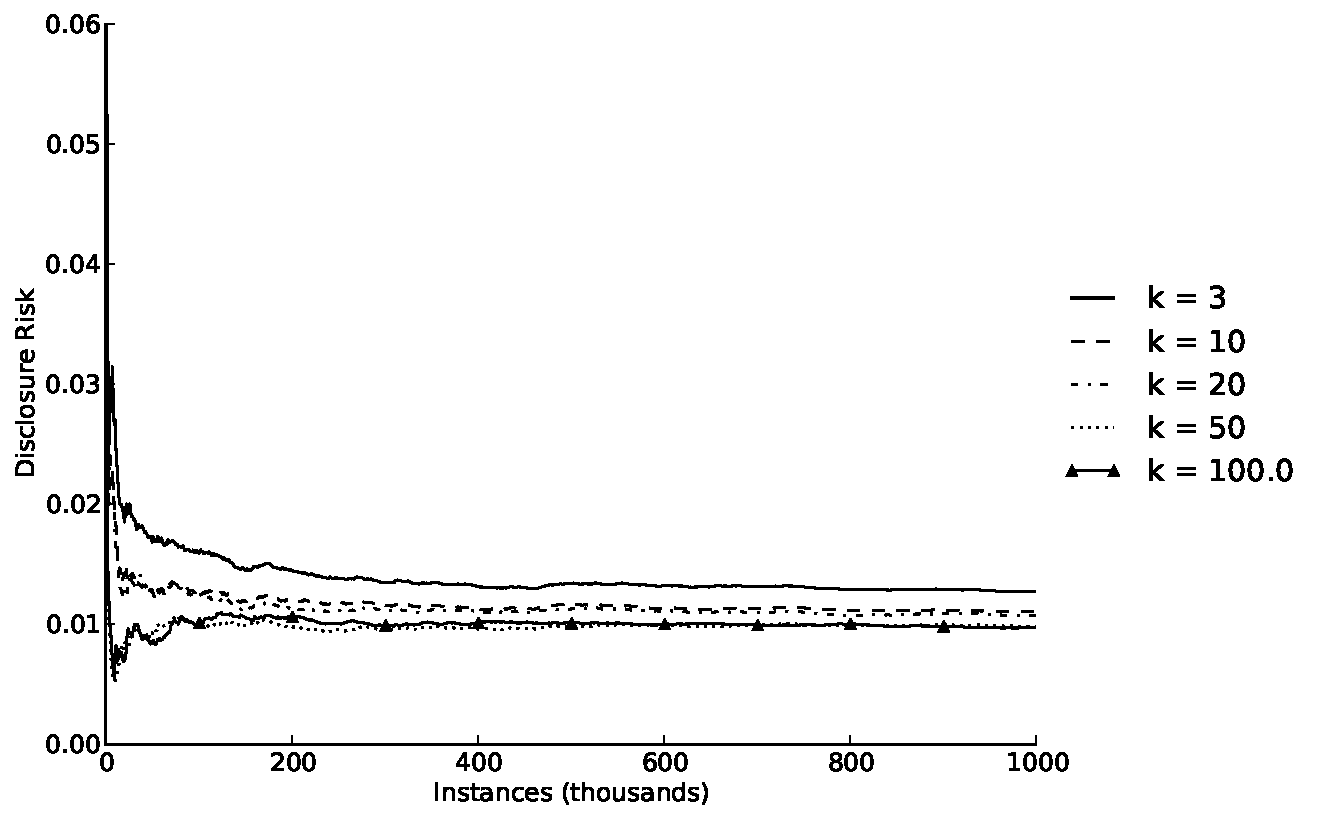
\includegraphics[width=0.9\linewidth]{figures/dr_dp-e1-random.pdf}
	\caption[Differential privacy DR evaluation ($b = 100,~\varepsilon = 1$).]{\texttt{DifferentialPrivacyFilter} DR evaluation using the \texttt{RandomRBFGenerator} with fixed buffer size $b = 100$ and fixed differential privacy scale parameter $\varepsilon = 1$, for increasing $k$.}
	\label{fig:results-dr-dp-e1}
\end{figure}

\begin{figure}[h]
	\centering
	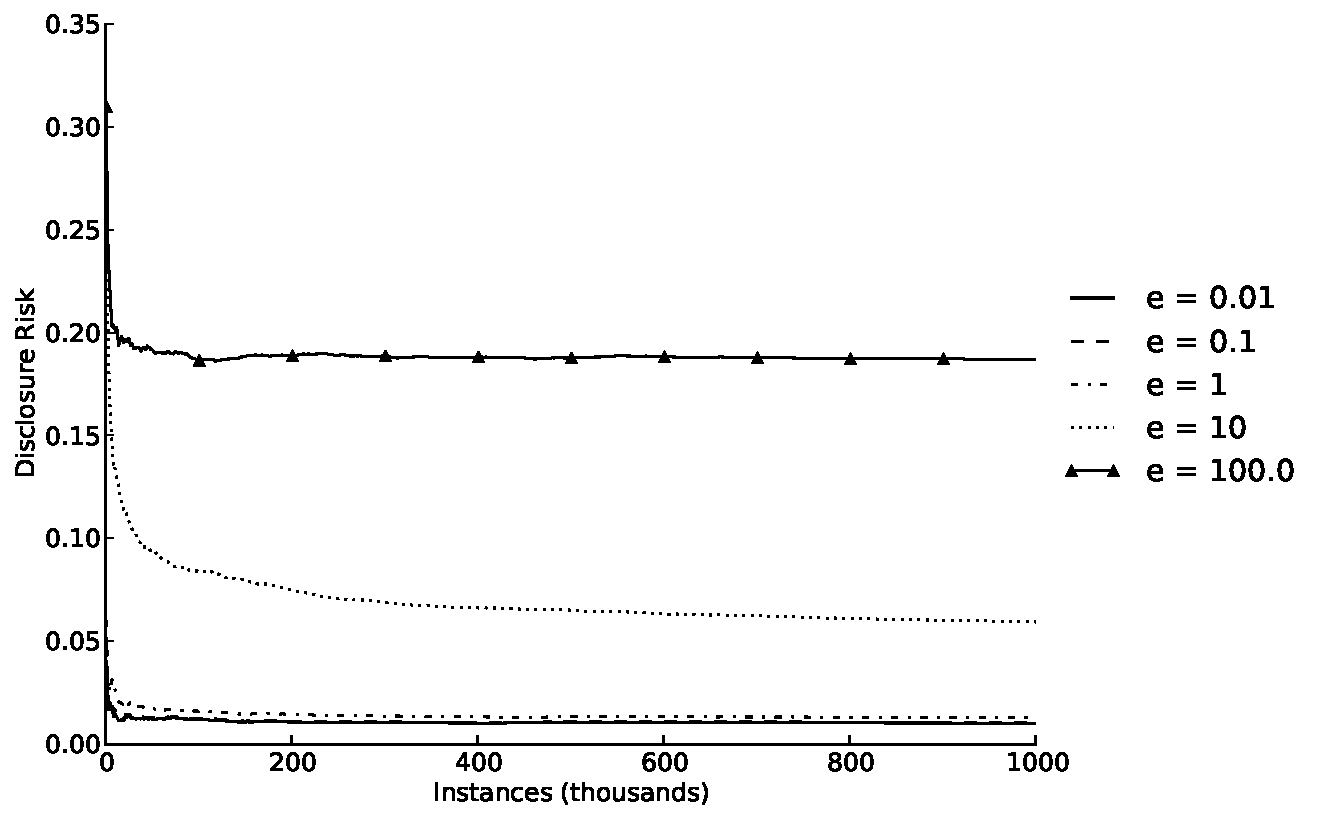
\includegraphics[width=0.9\linewidth]{figures/dr_dp-k3-random.pdf}
	\caption[Differential privacy DR evaluation ($b = 100,~k = 3$).]{\texttt{DifferentialPrivacyFilter} DR evaluation using the \texttt{RandomRBFGenerator} with fixed buffer size $b = 100$ and fixed cluster size $k = 3$, for increasing $\varepsilon$ differential privacy scale factor.}
	\label{fig:results-dr-dp-k3}
\end{figure}

\begin{figure}[h]
	\centering
	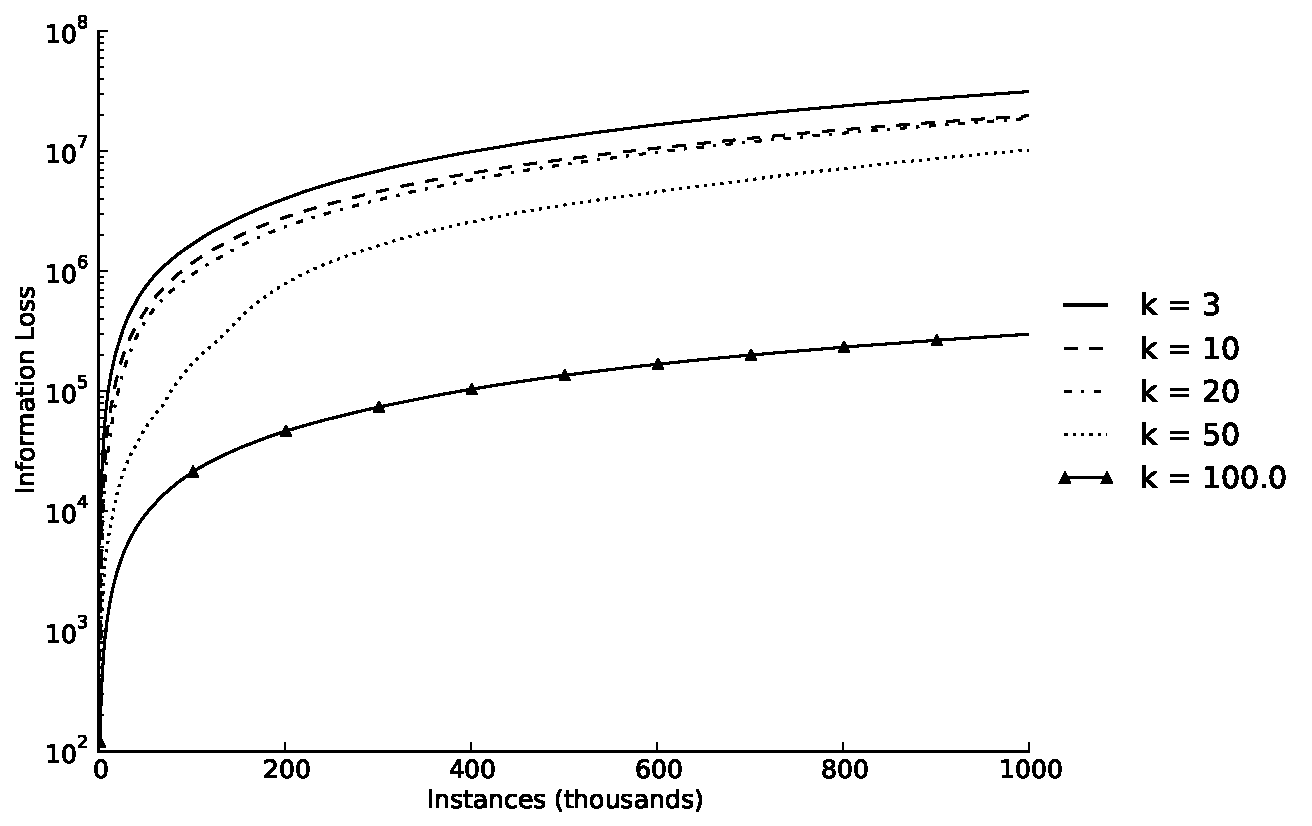
\includegraphics[width=0.9\linewidth]{figures/il-log_dp-e1-random.pdf}
	\caption[Differential privacy IL evaluation ($b = 100,~\varepsilon = 1$).]{\texttt{DifferentialPrivacyFilter} IL evaluation using the \texttt{RandomRBFGenerator} with fixed buffer size $b = 100$ and fixed differential privacy scale parameter $\varepsilon = 1$, for increasing $k$, on a logarithmic scale.}
	\label{fig:results-il-dp-e1}
\end{figure}

\begin{figure}[h]
	\centering
	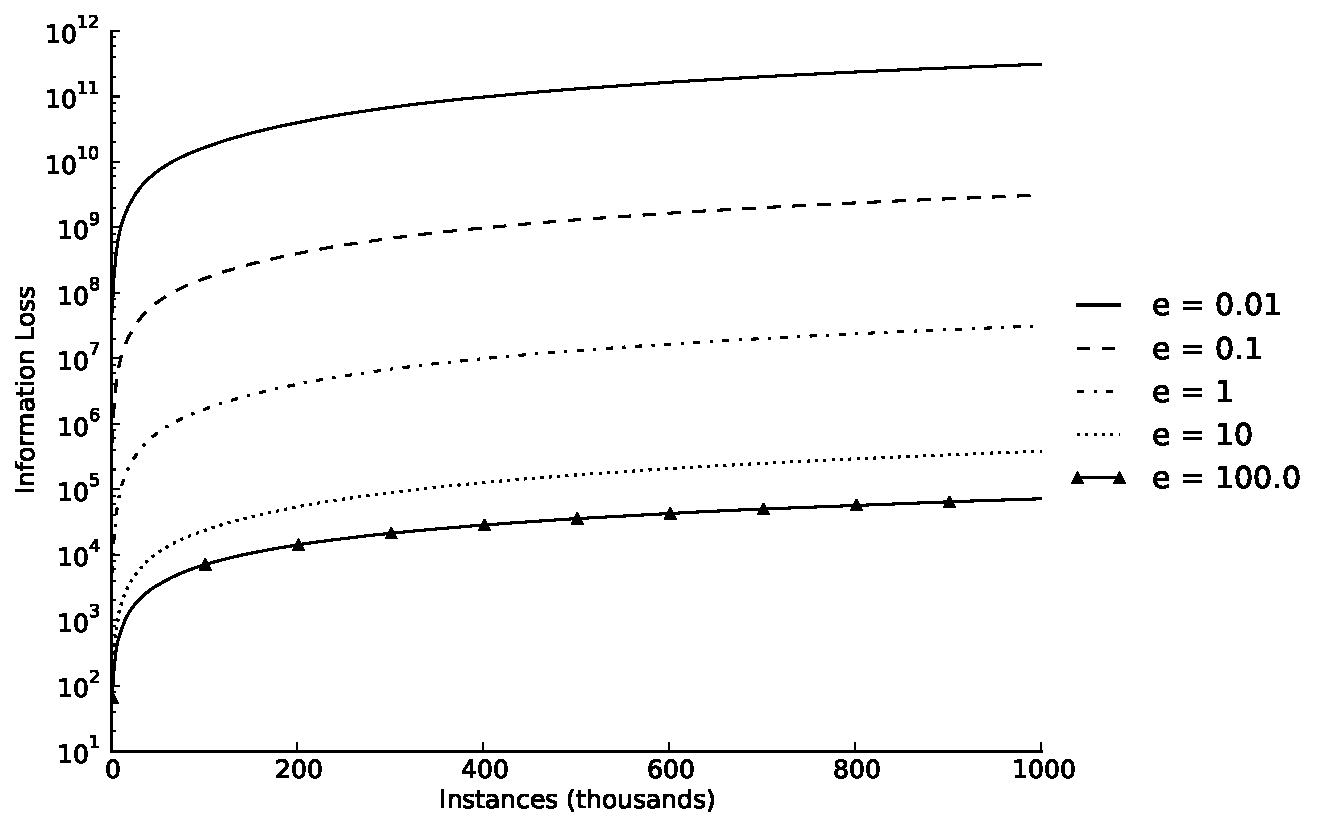
\includegraphics[width=0.9\linewidth]{figures/il-log_dp-k3-random.pdf}
	\caption[Differential privacy IL evaluation ($b = 100,~k = 3$).]{\texttt{DifferentialPrivacyFilter} IL evaluation using the \texttt{RandomRBFGenerator} with fixed buffer size $b = 100$ and fixed cluster size $k = 3$, for increasing $\varepsilon$ differential privacy scale factor, on a logarithmic scale.}
	\label{fig:results-il-dp-k3}
\end{figure}
